\documentclass[border=10pt]{standalone}
\usepackage{tikz}
\usepackage{amsmath}
\usetikzlibrary{calc,arrows.meta}
\begin{document}
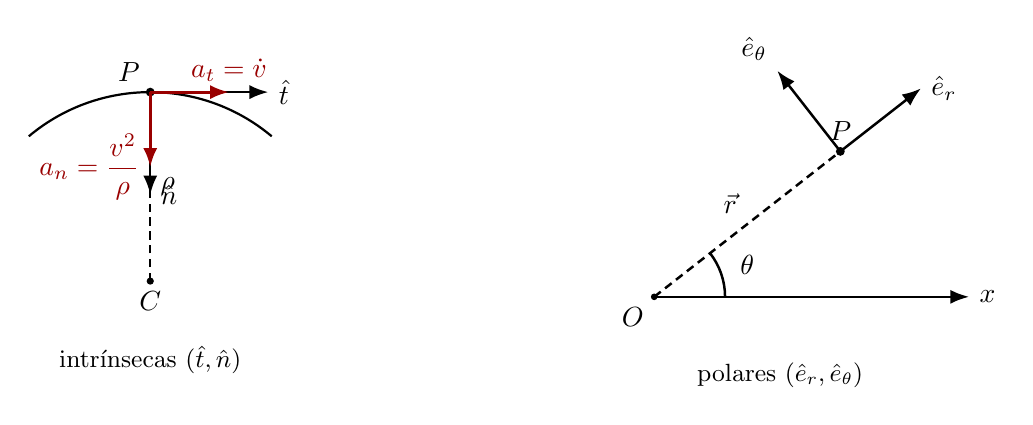
\begin{tikzpicture}[line width=0.9pt,>={Latex[length=2.4mm]}]
  % ===== Panel A: intrinsecas (t-n) =====
  \coordinate (C) at (0,0);
  \coordinate (P) at (0,2.4);
  \draw[thick] ([shift=(50:2.4)]C) arc (50:130:2.4);
  \draw[densely dashed] (C) -- (P) node[midway,right]{$\rho$};
  \fill (C) circle(1.3pt) node[below]{$C$};
  \fill (P) circle(1.6pt) node[above left]{$P$};
  % tangente (direccion del movimiento, +x)
  \draw[->] (P) -- ++(1.5,0) node[right]{$\hat t$};
  % normal (hacia C)
  \draw[->] (P) -- ++(0,-1.3) node[right]{$\hat n$};
  % aceleraciones
  \draw[->,red!60!black,line width=1.1pt] (P) -- ++(1.0,0) node[above]{$a_t=\dot v$};
  \draw[->,red!60!black,line width=1.1pt] (P) -- ++(0,-0.95) node[left]{$a_n=\dfrac{v^2}{\rho}$};
  \node at (0,-1.0){\small intrínsecas $(\hat t,\hat n)$};
  % ===== Panel B: polares =====
  \begin{scope}[xshift=6.4cm,yshift=-0.2cm]
    \coordinate (O) at (0,0);
    \coordinate (P2) at (38:3.0);
    \draw[->] (O) -- (4,0) node[right]{$x$};
    \draw[densely dashed] (O) -- (P2) node[midway,above left]{$\vec r$};
    \fill (O) circle(1.2pt) node[below left]{$O$};
    \fill (P2) circle(1.6pt) node[above]{$P$};
    \draw (0.9,0) arc (0:38:0.9); \node at (19:1.25){$\theta$};
    \draw[->] (P2) -- ($(P2)+(38:1.3)$) node[right]{$\hat e_r$};
    \draw[->] (P2) -- ($(P2)+(128:1.3)$) node[above left]{$\hat e_\theta$};
    \node at (1.6,-1.0){\small polares $(\hat e_r,\hat e_\theta)$};
  \end{scope}
\end{tikzpicture}
\end{document}
